\documentclass[a4paper,11pt,hidelinks]{article}
\usepackage[utf8]{inputenc}  % Linux, macOS: enable non-English characters
%\usepackage[latin1]{inputenc}    % Windows: enable non-English characters
\usepackage[british]{babel}
\usepackage{fullpage}

\usepackage{amsmath}
\usepackage{amssymb}
\usepackage{amsthm} \newtheorem{theorem}{Theorem}
\usepackage{booktabs}
%\usepackage{clrscode4e}
\usepackage{color}
\usepackage{courier} % \texttt{...} gives thinner text
\usepackage{float}
\usepackage{mathtools} % provides \coloneqq
\usepackage{multirow}
\usepackage{soul} % provides \st for overstriking
\usepackage{tikz} \usetikzlibrary{trees}
\usepackage{xspace}
\usepackage{hyperref}  % should always be the last package

\newcommand{\deleted}[1]{{\color{red}\st{#1}}}  % deleted text in strike-out red
\newcommand{\todo}[1]{{\color{blue}#1}}  % to-do items in blue
%\newcommand{\todo}[1]{#1}               % to-do items in black
\newcommand{\done}[1]{{\color{red}#1}}   % new/revised text in red
%\newcommand{\done}[1]{#1}               % new/revised text in black

\newcommand{\filler}{$\Tuple{\dots}$}    % place holder for student text

%% useful (wrappers for) math symbols:
\newcommand{\Cardinality}[1]{\left\lvert#1\right\rvert}
%\newcommand{\Cardinality}[1]{\##1}
\newcommand{\Ceiling}[1]{\left\lceil#1\right\rceil}
\newcommand{\Floor}[1]{\left\lfloor#1\right\rfloor}
\newcommand{\Iff}{\Leftrightarrow}
\newcommand{\Implies}{\Rightarrow}
\newcommand{\Intersect}{\cap}
\newcommand{\Oh}[1]{\mathcal{O}\left(#1\right)}
\newcommand{\Sequence}[1]{\left[#1\right]}
\newcommand{\Set}[1]{\left\{#1\right\}}
\newcommand{\SetComp}[2]{\Set{#1\SuchThat#2}}
\newcommand{\SuchThat}{\mid}
\newcommand{\Tuple}[1]{\langle#1\rangle}
\newcommand{\twodots}{\mathinner{\ldotp\ldotp}}  % taken from clrscode3e.sty
\newcommand{\Union}{\cup}

%% fancy characters:
\usepackage{pifont}
%\newcommand{\scissors}{\ding{36}}
%\newcommand{\phone}{\ding{37}}
%\newcommand{\aircraft}{\ding{40}}
%\newcommand{\envelope}{\ding{41}}
\newcommand{\handpoint}{\ding{43}}
%\newcommand{\victory}{\ding{44}}
%\newcommand{\handwrite}{\ding{45}}
%\newcommand{\tick}{\ding{51}}
%\newcommand{\notick}{\ding{55}}

\title{\textbf{Algorithms and Data Structures III (course 1DL481) \\
    Uppsala University -- Spring 2024 \\
    Report for Assignment \todo{n}  %% Replace n by 1 or 2
    by Team \todo{t}}}              %% Replace t by your team number

%% Replace by your name(s) and choose the encoding of line 2 or line 3:
\author{\todo{Clara CLÄVER} \and \todo{Whiz KIDD}}

%\date{Month Day, Year}
\date{\today}

\begin{document}

\maketitle

\todo{
  %% Delete this paragraph:
  \noindent
  This document imposes the \emph{structure} of an assignment report
  for this course.  The \LaTeX\ source code of this document
  exemplifies almost everything you need to know about \LaTeX\ in
  order to typeset a professional-looking assignment report (for this
  course).  Use it as a starting point for imitation and delete
  everything irrelevant.  The usage of \LaTeX\ is \emph{optional}, but
  highly recommended, for reasons that will soon become clear to those
  who have never used it before: any learning time is \emph{outside}
  the budget of this course, but will hugely pay off, if not in this
  course then in the next course(s) you take and when writing a thesis
  or other scientific report. \medskip

  %% Delete this paragraph:
  Replace every blue text by your text (or just delete it, where
  appropriate, such as this and the preceding paragraphs) and drop the
  call to the \texttt{\textbackslash{}todo} command, so that its
  argument appears in black.
  
}

%% Comment away for Assignment 2:
\section*{Problem 1: Mixed Integer Programming (MIP)}

%% Fix below and drop the invocation of the \todo command:
\newcommand{\SolverMIP}{\todo{Gurobi}\xspace}  % or CPLEX, or Xpress, or Cbc
\newcommand{\TimeoutMIP}{\todo{300.00}}  % timeout, in CPU seconds; MIN 300.00

\paragraph{Task~a: Model.}~
\todo{What are the variables, their meanings, their constraints, and
  the objective function?
  % 
  For example, for the investment design problem, one might write:
  ``Let variable~$m_{ij}$ take value~$1$ if basket~$i$ invests in
  credit~$j$, and value~$0$ otherwise, with $i \in 1 \twodots v$ and
  $j \in 1 \twodots b$.
  % 
  The constraint that each row must sum up to~$r$ can then be linearly
  modelled as
  \[
    \forall i \in 1 \twodots v : \sum_{j \in 1 \twodots b} m_{ij} = r
  \]
  % 
  Etc.''
  %
}

\paragraph{Task~b: Implementation.}
Our model \texttt{servStatLoc.mod} is \todo{uploaded} with this report
(but not listed inside it): we \todo{checked} that its constraints and
objective function are linear (and we are aware that four points will
otherwise be deducted from our score for this problem).
%
We chose the MIP solver~\SolverMIP for our experiments, which we ran
\todo{on the NEOS server or
  % specification of the ThinLinc Linux hosts of the IT department,
  % where the academic site license for Gurobi is installed, but note
  % that no classroom license for AMPL is installed there, so replace
  % if need be by a similar-looking specification of your own hardware:
  under Linux Ubuntu~18.04 ($64$~bit) on an Intel Xeon E5520 of
  $2.27$~GHz, with $4$~processors of $4$~cores each, with a $70$~GB
  RAM and an $8$~MB L3 cache (a ThinLinc computer of the IT
  department)}.

\paragraph{Task~c: 10 Zones.}
The results are in Table~\ref{tab:res:mip}.
%% not needed from vt24 on:
% When~$s$ increases, the optimal objective value~\todo{\filler}.

\paragraph{Task~d: 20 Zones.}
The results are in Table~\ref{tab:res:mip}.
%% not needed from vt24 on:
% When~$s$ grows beyond~$4$, the optimal objective value \todo{\filler}.

\paragraph{Task~e: 40 Zones.}
The results are in Table~\ref{tab:res:mip}.

\paragraph{Task~f: 80 Zones.}
The results are in Table~\ref{tab:res:mip}.
%% not needed from vt24 on:
% Upon~$s=16$ service stations with~$v=1$ vehicle each, the optimal
% objective value is \todo{\filler} the one for~$s=8$ and~$v=2$, because
% \todo{\filler}.

\paragraph{Task~g: 120 Zones.}
The results are in Table~\ref{tab:res:mip}.
%
Our model \todo{does not time out}.
%% If it does time out, then see the demo sentence under Task h below!

\paragraph{Task~h: 250 Zones.}
The results are in Table~\ref{tab:res:mip}.
%
Our model \todo{times out, so our proposed algorithm for delivering a
  not necessarily optimal solution in reasonable running time is
  \filler}.

\paragraph{Task~i: Brute-Force Algorithm.}
The size of the search space of a totally brute-force search algorithm
is \todo{$\binom{z!}{\cos c} \cdot \log_s v$}, because \todo{\filler}.

The numbers of candidate solutions this brute-force search algorithm
has to examine per second in order to match the reported runtime
performance of~\SolverMIP on our model are given in the right-most
column of Table~\ref{tab:res:mip}, for each instance that~\SolverMIP
solved to proven optimality without timing out.
%
%% not needed from vt24 on:
% We think that \todo{\filler}, because \todo{\filler}.

\begin{table}[t]  % make it float to the top of a page
  \centering
  \begin{tabular}{rrrrrrrr}  % right alignment --> decimal point alignment
    $z$ & $s$ & $v$ & $c$ & time & objective value & optimality gap & brute-force \\
    \midrule
    % Make sure every number in a column has the _same_ number of decimals,
% so as to get decimal-point alignment and easy comparison of numbers!
%
% Witness in particular the 0.023246261350 instead of 0.02324626135 in line 4!
%
 10 &  2 & 2 & 3 &  \todo{67.89} & 0.008740338682 & 0.00\% & \todo{$10^{17}$} \\
 10 &  3 & 2 & 3 \\
 10 &  4 & 2 & 3 \\
 20 &  2 & 2 & 3 & \todo{123.45} & 0.023246261350 & 0.00\% & \todo{$10^{23}$} \\
 20 &  3 & 2 & 3 \\
 20 &  4 & 2 & 3 \\
 20 &  5 & 2 & 3 \\
 20 &  6 & 2 & 3 \\
 40 &  5 & 2 & 3 \\
 80 &  8 & 2 & 3 \\
 80 & 16 & 1 & 3 \\
120 & 10 & 2 & 3 \\
250 & 12 & 3 & 4 & \TimeoutMIP & & \todo{2.34\%} & \todo{n/a} \\
 %% let your experiment script write directly
                            %% into this file, making sure every number
                            %% in a column has the _same_ number of decimals
  \end{tabular}
  \caption{Service station location: runtime (in seconds), objective
    value, and optimality gap (in percent; positive if an optimal
    solution was not found and proven before timing out)
    using~\SolverMIP, with a timeout of $\TimeoutMIP$~CPU seconds.
    The right-most column gives the number of candidate solutions the
    brute-force search algorithm has to examine per second in order to
    match the runtime performance of~\SolverMIP, if the instance was
    solved to proven optimality, and~`n/a' for `non-applicable'
    otherwise.
    %% delete the following sentence:
    \todo{(The sample performance of this demo report is made up,
      but the two optimal objective values are correct!)}
    % 
  }
  \label{tab:res:mip}
\end{table}

%%% Local Variables:
%%% mode: latex
%%% TeX-master: "demoReport"
%%% End:


%% Comment away for Assignment 2:
\clearpage
\section*{Problem 2: Stochastic Local Search (SLS)}

\todo{
  %% delete this paragraph, including its footnote:
  The \emph{investment design problem} is about finding a matrix of
  $v$~rows and $b$~columns of~$0$-$1$ integer values, such that each
  row sums up to~$r$, with $v \geq 2$ and $b \geq r \geq 1$, and the
  largest dot product between all pairs of rows is minimised.
  % 
  Equivalently, one has to find~$v$ subsets of size~$r$ within a given
  set of $b$~elements, such that the largest intersection of any two
  of the $v$~sets has minimal size.
  % 
  An instance of the problem is parametrised by a
  triple~$\Tuple{v,b,r}$.\footnote{\todo{Your report need not contain
      an explanation of the problem to be solved: you can assume the
      reader has read the problem statement in the assignment
      instructions.  We just repeat it here for self-sufficiency of
      this document.}}
  
  %% delete this paragraph:
  This is an abstract description of a problem that appears in
  finance: see Figure~\ref{fig:wallStreet}.  In a typical investment
  design in finance, we have $4 \leq v \leq 25$ and
  $250 \leq b \leq 500$, with $r \approx 100$.

  %% delete this figure:
  \begin{figure}[b]  % make it float to the bottom of a page
    \centering
    \includegraphics[height=5cm]{wallStreet}
    \caption{\todo{Wall Street (\copyright\ www.forbes.com, 2014)}}
    \label{fig:wallStreet}
  \end{figure}
  
  %% delete this paragraph, if you want:
  A lower bound on the number~$\lambda$ of shared elements of any
  pair among $v$~subsets of size~$r$ drawn from a given set of
  $b$~elements is given in~\cite{ASTRA:AOC}:
  \begin{equation}\label{eq:lb}
  \text{lb}(\lambda) = 
    \Ceiling{
      \frac{\Ceiling{\frac{rv}{b}}^{2} ((rv) \bmod b)  +
        \Floor{\frac{rv}{b}}^{2} (b - ((rv) \bmod b)) - rv}
      {v(v-1)}
    }
  \end{equation}
  
}

\paragraph{Task~a: SLS Algorithm.}
\begin{enumerate}
\item Representation.  \todo{Describe how to represent the problem:
  what are the variables, their meanings, their constraints, and the
  objective function?}
\item Initial Assignment.  \todo{Describe an algorithm for generating
  (fast) a randomised initial assignment.}
\item Move.  \todo{Describe one or more moves that go from an
  assignment to a neighbouring assignment by changing the values of
  a few variables.}
\item Constraints.  \todo{Describe for each constraint how its
  satisfaction is either algorithmically checkable efficiently or
  guaranteed to be preserved by the previous two design choices.}
\item Neighbourhood.  \todo{Describe a neighbourhood based on the
  proposed moves.
  % 
  Derive a formula for computing the size of the neighbourhood in
  terms of the problem parameters.
  % 
  Discuss whether the neighbourhood makes the search space connected,
  in the sense that every feasible assignment (that is, every
  assignment satisfying all the constraints, whether optimal or not)
  is reachable from every initial assignment (you only need to sketch
  a proof if the search space is connected, and give a counterexample
  otherwise).}
\item Cost Function.  \todo{Describe a cost function, whose value is
  to be minimised during search.}
\item Probing.  \todo{Describe how a neighbouring assignment, as
  reachable by a move, can be probed efficiently:
  % 
  describe how the cost function can be evaluated efficiently and
  incrementally, and describe the data structures used to do so.
  % 
  Give, without proof, the time complexity of probing; ideally, it is
  (sub-)linear in the problem parameters.}
\item Heuristic.  \todo{Describe a heuristic for exploring (via
    probing) the neighbourhood and selecting a neighbouring assignment
    to commit to.
  % 
  State whether the neighbourhood is explored exhaustively and, if
  so, how you determine when it was exhausted.
  % 
  Explain how you ensure that the same neighbour is not probed twice
  during a given exploration.}
\item Optimality.  \todo{Describe how you use a bound on the objective
  value in order to terminate sometimes the search with proven
  optimality, as part of the heuristic.}
\item Meta-Heuristic.  \todo{Describe a meta-heuristic based on tabu
  search: explain how the tabu list is represented; choose (a
  formula for) its size; explain how fine-grained its content is;
  and describe how it can be looked up and maintained efficiently;
  note that the tabu list is not necessarily an actual list, but
  rather a concept; make sure that worsening moves are sometimes
  made.}
\item Random Restarts.  \todo{Describe how to detect or guess that a
  random restart should be made, as part of the meta-heuristic.}
\item Optional Tweaks.  \todo{Describe ideas that you used in order to
  improve your algorithm.}
\end{enumerate}
In summary, the local-search parameters (not the problem
parameters~$v$,~$b$,~$r$) are~\todo{$\alpha$ and~$\beta$.}

\paragraph{Task~b: Implementation.}
We chose the high-performance programming language \todo{Java}, for
which a \todo{compiler or interpreter} is available on the Linux
computers of the IT department.  All source code is \todo{uploaded}
with this report (but not listed inside it).  The compilation and
running instructions are \todo{\filler}.

An executable called \texttt{InvDes} reads the problem
parameters~$v$,~$b$,~$r$ as command-line arguments and writes to
standard output a line with the space-separated values
of~$v$,~$b$,~$r$, the lower bound~$\text{lb}(\lambda)$ on~$\lambda$,
and the achieved~$\lambda$, followed by one line per row of
a~$v \times b$ matrix representing the solution, the~$0$-$1$ cell
values being space-separated.

We validated the correctness of our implementation by \todo{checking
  its outputs on 1,258 instances via the provided polynomial-time
  solution checker}.

\paragraph{Task~c: Experiments.}
%% Note the non-breaking spaces, typeset via ~, between numbers and
%% their units:
All experiments were run under
% specification of the ThinLinc machines of the IT department, or
% replace by a similar-looking specification of your own hardware:
\todo{Linux Ubuntu~18.04 ($64$~bit) on an Intel Xeon E5520 of
  $2.27$~GHz, with $4$~processors of $4$~cores each, with a $70$~GB
  RAM and an~$8$~MB L3 cache (a ThinLinc computer of the IT
  department).}

We fine-tuned the local-search parameters as follows.  \todo{Discuss
  the impact of the local-search parameters~$\alpha$ and~$\beta$ on
  the performance of your SLS algorithm.}

\newcommand{\TimeoutSLS}{\todo{300.0}}  % timeout, in CPU seconds; MIN 300.0
\newcommand{\RunsSLS}{\todo{5}}         % independent runs per instance; MIN 5

The \todo{median} runtime (in seconds), \todo{median} number of steps,
and \todo{median} achieved~$\lambda$ over~$\RunsSLS$ independent runs
for each of the $21$~instances of the assignment instructions are
given in Table~\ref{tab:res:sls}, for \todo{two} configurations
%% remember: AT LEAST TWO, except for solo teams!
of values for the local-search parameters~\todo{$\alpha$ and~$\beta$}.
The timeout was~$\TimeoutSLS$~CPU seconds per run.%
%
%% Delete this footnote:
\footnote{\todo{Hint: In order to save a lot of time, it is very
    important that you write a script that conducts the experiments
    for you and directly generates a result table (see the \LaTeX\
    source code of Table~\ref{tab:res:sls} for how to do that), which
    is then automatically imported, rather than manually copied, into
    your report: each time you change the code, it suffices to re-run
    that script and re-compile your report, without any tedious
    copying!  The sharing of scripts is allowed and even encouraged.}}

\begin{table}[t]  % make it float to the top of a page
  \centering
  \begin{tabular}{rrrrrrrrrrr}  % right alignment --> decimal point alignment
    & & &
    & \multicolumn{3}{c}{\todo{$\Tuple{\alpha,\beta}=\Tuple{10,5}$}}
    & \multicolumn{3}{c}{\todo{$\Tuple{\alpha,\beta}=\Tuple{20,8}$}} \\
    \cmidrule(r){5-7} \cmidrule(r){8-10}
    $v$ & $b$ & $r$ & $\text{lb}(\lambda)$
        & time & steps & $\lambda$
        & time & steps & $\lambda$ & exact \\
    \midrule
    % Make sure every number in a column has the _same_ number of decimals,
% so as to get decimal-point alignment and easy comparison of numbers!
%
% Witness in particular the 300.0 instead of 300!
%
10 &  30 &   9 &  2 & 300.0 &  123 & 3 &  45.0 &  678 & 2 & $10^{22}$ \\
12 &  44 &  11 &  2 & 300.0 &  901 & 3 & 234.5 & 5678 & 2 & $10^{21}$ \\
15 &  21 &   7 &  2 & 300.0 & 1023 & 4 & 300.0 & 6789 & 3 &      n/a \\
16 &  16 &   6 &  2 & 123.4 &  567 & 2 &  89.1 & 2345 & 2 & $10^{14}$ \\
 9 &  36 &  12 &  3 \\
11 &  22 &  10 &  4 \\
19 &  19 &   9 &  4 \\
10 &  37 &  14 &  5 \\
 8 &  28 &  14 &  6 \\
10 & 100 &  30 &  7 \\
 6 &  50 &  25 & 10 \\
 6 &  60 &  30 & 12 \\
11 & 150 &  50 & 14 \\
 9 &  70 &  35 & 16 \\
10 & 350 & 100 & 22 \\
13 & 250 &  80 & 22 \\
10 & 325 & 100 & 24 \\
15 & 350 & 100 & 24 \\
 9 & 300 & 100 & 25 \\
12 & 200 &  75 & 25 \\
10 & 360 & 120 & 32 \\
 %% let your experiment script write directly
                            %% into this file, making sure every number
                            %% in a column has the _same_ number of decimals
  \end{tabular}
  \caption{Investment design: median runtime (in seconds), median
    number of steps, and median achieved~$\lambda$, for \todo{two}
    configurations
    %% remember: AT LEAST TWO, except for solo teams!
    of values for the local-search parameters~\todo{$\alpha$
      and~$\beta$}, over~$\RunsSLS$~independent runs per instance,
    with a timeout of $\TimeoutSLS$~CPU seconds per run.
    %
    The right-most column gives the number of candidate solutions the
    outlined exact algorithm has to examine per second in order
    to match the runtime performance of the seemingly best
    configuration of values for the local-search parameters, namely
    \todo{$\Tuple{\alpha,\beta}=\Tuple{20,8}$}, if the instance
    was solved to proven optimality, and `n/a' for `non-applicable'
    otherwise.
    %% delete the following sentence:
    \todo{(The sample performance of this demo report is made up!)}
    %
  }
  \label{tab:res:sls}
\end{table}

We observe that \todo{\filler}, because \todo{\filler}.

\paragraph{Task~d: Exact Algorithm.}
An exact algorithm could work as follows: \todo{discuss its features
  (for instance, does it perform brute-force search?).}
%
The size of the search space of this exact algorithm is
\todo{$\binom{r!}{\cos b} \cdot \log v$}, because \todo{\filler}.

The number of candidate solutions this exact algorithm has to examine
per second in order to match the runtime performance of the seemingly
best configuration of values for the local-search parameters,
according to Task~c, of our stochastic local search algorithm is given
in the right-most column of Table~\ref{tab:res:sls}, for each instance
solved to proven optimality.
%
We think that \todo{\filler}, because \todo{\filler}.

%%% Local Variables:
%%% mode: latex
%%% TeX-master: "demoReport"
%%% End:


%% Comment away for Assignment 1:
\clearpage
\section*{Problem 3: Boolean Satisfiability (SAT)}

\newcommand{\MiniSat}{Mini\-Sat}  % avoids default hyphenation into Min-iSat
%% Fix below and drop the invocation of the \todo command:

\newcommand{\SolverSAT}{\todo{\MiniSat}\xspace}  % or Lingeling, or ...
\newcommand{\TimeoutSAT}{\todo{60.0}}  % timeout, in CPU seconds; MIN 60.0

\paragraph{Task~a: Ordered Resolution.}
Consider the following formula in conjunctive normal form (CNF):
\begin{multline*}
  \varphi \equiv (x_1 \lor x_2) \land
  (x_3 \lor x_4) \land
  (x_5 \lor x_6) \land
  (\neg x_1 \lor \neg x_3) \land
  (\neg x_1 \lor \neg x_5) \\ \land
  (\neg x_3 \lor \neg x_5) \land
  (\neg x_2 \lor \neg x_4) \land
  (\neg x_2 \lor \neg x_6) \land
  (\neg x_4 \lor \neg x_6)
\end{multline*}
\todo{Perform ordered resolution
  % (cf.\ \emph{Introduction to SAT}, slide~19)
  on this formula, selecting the variables in the order given by their
  index (i.e., $x_1$ before $x_2$ before~\dots).  Show the result
  after each iteration.
  % 
  Based on your resolution, is~$\varphi$ satisfiable?
}

\paragraph{Task~b: DPLL.}
Consider again the formula~$\varphi$ given in Task~a.
% 
\todo{Explain in detail how the DPLL algorithm,
  % (cf.\ \emph{Introduction to SAT}, slide~26),
  when applied to~$\varphi$, determines whether the formula is
  satisfiable.
  % 
  Assume that the variables are selected in the order given by their
  index (i.e., $x_1$ before $x_2$ before~\dots), and that they are
  assigned~$1$ (i.e., True) before they are assigned~$0$ (i.e.,
  False).
  % 
  Remember to perform unit propagation and to apply the pure-literal
  rule where possible, in order to prune parts of the search space.
}

\paragraph{Task~c: CDCL.}
Consider the following CNF formula:
\[
  (x_1 \lor x_8 \lor \neg x_2) \land
  (x_1 \lor \neg x_3) \land
  (x_2 \lor x_3 \lor x_4) \land
  (\neg x_4 \lor \neg x_5) \land
  (x_7 \lor \neg x_4 \lor \neg x_6) \land
  (x_5 \lor x_6)
\]
Assume that~$x_7$ has been assigned~$0$ at decision level~$2$, and
that~$x_8$ has been assigned~$0$ at decision level~$3$.
% 
Moreover, assume that the current decision assignment is $x_1 = 0$ at
decision level~$5$.
% 
\todo{Draw a resulting implication graph (possibly on paper or a
  whiteboard, and include it using the syntax for
  Figure~\ref{fig:wallStreet}).
  %% See \emph{Mini-tutorial on conflict-driven clause learning
  %% solvers}, slide~4.
  %
  % \begin{figure}[t]  % make it float to the top of a page
  %   \centering
  %   \includegraphics[height=5cm]{implicationGraph.jpg}
  %   \caption{An implication graph for Task~c}
  %   \label{fig:impGraph}
  % \end{figure}
  Does the graph contain any conflicts?  If so, then mark these
  clearly, and provide a conflict clause.
}

\paragraph{Task~d: Encoding.}~ \todo{Describe your encoding, citing
  either~\cite{AMK:CNF:Sinz}, or~\cite[Section~2.2.2]{CNFencodings},
  or both, if you use their ideas: first explain the meaning of the
  Boolean variables that you use in your formula~$\varphi_{d,c,e}$;
  then explain the encodings by the help functions
  % $\textsc{AndImply}(x_1,\dots,x_n,b)$ and
  % $\textsc{OrImply}(x_1,\dots,x_n,b)$
  of the hint that you actually use (there is no need to explain
  $\textsc{AtMost}(k,x_1,\dots,x_n)$ if you use~\cite{AMK:CNF:Sinz});
  and finally explain how the constraints of the problem are encoded
  using those variables and help functions.}

We chose the programming language \todo{\filler}, for which a compiler
or interpreter is available on the Linux computers of the IT
department.  All source code is \todo{uploaded} with this report (but
not listed inside it).  The compilation and running instructions are
\todo{\filler}.

We validated the correctness and speed of our encoding by
\todo{checking its outputs on 1,258 instances via the provided
  polynomial-time solution checker and by judging the runtime to be
  short}.

\paragraph{Task~e: Experiments.}
We chose the SAT solver \SolverSAT for our experiments.
%
We \todo{used or did not use} the provided script for running the
experiments and tabling their results
% specification of the ThinLinc machines of the IT department, or
% replace by a similar-looking specification of your own hardware:
\todo{under Linux Ubuntu~18.04 ($64$~bit) on an Intel Xeon E5520 of
  $2.27$~GHz, with $4$~processors of $4$~cores each, with a $70$~GB
  RAM and an $8$~MB L3 cache (a ThinLinc computer of the IT
  department)}.
% on the AD3 web interface to \MiniSat on a $2.69$~GHz Intel
% Core i7, with $8$~GB RAM and $4$~MB L3 cache.

The results are in Table~\ref{tab:res:sat}.
%
The trivially unsatisfiable instances (which are the ones that violate
the inequality $e \leq \Floor{\frac{d-1}{c-1}}$) that \todo{were
  actually attempted in our experiments} are
%% In other words: delete the ones that are NOT in YOUR table, and add
%% the missing ones that ARE in YOUR table:
$\Tuple{8,2,8}$, $\Tuple{10,2,10}$, $\Tuple{12,2,12}$,
$\Tuple{14,2,14}$, $\Tuple{16,2,16}$, $\Tuple{15,3,8}$,
\todo{\filler}, $\Tuple{16,4,6}$, \todo{\filler}, and \todo{\filler}.
%
We observe that our encoding detects their trivial unsatisfiability in
\todo{\filler} time.

\begin{table}[t]  % make it float to the top of a page
  \centering
  \begin{tabular}{rrrrr}  % right alignment --> decimal point alignment
$d$ & $c$ & $e$ & status & time \\
\midrule
 8 & 2 &  7 &   sat &  \\
 8 & 2 &  8 & unsat &  \\ % trivially
10 & 2 &  9 &   sat &  \\
10 & 2 & 10 & unsat &  \\ % trivially
12 & 2 & 11 &   sat &  \\
12 & 2 & 12 & unsat &  \\ % trivially
14 & 2 & 12 &   sat &  \\
14 & 2 & 13 &   sat &  \\
14 & 2 & 14 & unsat &  \\ % trivially
16 & 2 & 10 &   sat &  \\
16 & 2 & 11 &   sat &  \\
16 & 2 & 12 &   sat &  \\
16 & 2 & 13 &   sat &  \\
16 & 2 & 14 &   sat &  \\
16 & 2 & 15 &   sat &  \\
16 & 2 & 16 & unsat &  \\ % trivially
\end{tabular}
~~
\begin{tabular}{rrrrr}
$d$ & $c$ & $e$ & status & time \\
\midrule
12 & 3 &  4 &   sat &  \\
12 & 3 &  5 & unsat &  \\ % not trivially!
15 & 3 &  6 &   sat &  \\
15 & 3 &  7 &   sat &  \\
15 & 3 &  8 & unsat &  \\ % trivially
18 & 3 &  6 &   sat &  \\
18 & 3 &  7 &   sat &  \\
18 & 3 &  8 &     ? &  \\
21 & 3 &  6 &   sat &  \\
21 & 3 &  7 &   sat &  \\
21 & 3 &  8 &   sat &  \\
21 & 3 &  9 &     ? &  \\
24 & 3 &  6 &   sat &  \\
24 & 3 & \dots& sat &  \\
24 & 3 &  9 &   sat &  \\
24 & 3 & 10 &     ? &  \\
\end{tabular}
~~
\begin{tabular}{rrrrr}
$d$ & $c$ & $e$ & status & time \\
\midrule
16 & 4 &  5 &   sat &  \\
16 & 4 &  6 & unsat &  \\ % trivially
20 & 4 &  4 &   sat &  \\
20 & 4 &  5 &   sat &  \\
20 & 4 &  6 &     ? &  \\
24 & 4 &  4 &   sat &  \\
24 & 4 &  5 &   sat &  \\
24 & 4 &  6 &     ? &  \\
28 & 4 &  4 &   sat &  \\
28 & 4 &  5 &   sat &  \\
28 & 4 &  6 &   sat &  \\
28 & 4 &  7 &     ? &  \\
32 & 4 &  3 &   sat &  \\
32 & 4 & \dots& sat &  \\
32 & 4 &  9 &   sat &  \\
32 & 4 & 10 &   sat &  
\end{tabular}

  \caption{Cruise design: satisfiability and runtime (in seconds)
    using \SolverSAT, with a timeout of $\TimeoutSAT$~CPU seconds; a
    timeout is denoted by~`t/o'; if no timeout occurred, then proven
    satisfiability is denoted by `sat' and proven unsatisfiability by
    `unsat', else trivial unsatisfiability is denoted by `unsat' and
    the unknown status is denoted by~`?'.}
  \label{tab:res:sat}
\end{table}

%%% Local Variables:
%%% mode: latex
%%% TeX-master: "demoReport"
%%% End:


%% Comment away for Assignment 1:
\clearpage
\section*{Problem 4: SAT Modulo Theories (SMT)}

%% Fix below and drop the invocation of the \todo command:
\newcommand{\SolverSMT}{\todo{Z3}\xspace}  % or CVC4, or Yices2, or ...
\newcommand{\TimeoutSMT}{\todo{60.0}}  % timeout, in CPU seconds; MIN 60.0 

\newcommand{\SASM}{\textsf{MiniASM}\xspace}
\newcommand{\Instr}[1]{\mathsf{#1}}
\newcommand{\Cmp}[1]{\Instr{cmp}_{#1}}
\newcommand{\Dup}{\Instr{dup}}
\newcommand{\Jmp}[1]{\Instr{jmp}_{#1}}
\newcommand{\Neg}{\Instr{neg}}
\newcommand{\Plus}{\Instr{plus}}
\newcommand{\Pop}{\Instr{pop}}
\newcommand{\Push}[1]{\Instr{push}_{#1}}
\newcommand{\Read}{\Instr{read}}
\newcommand{\Swap}{\Instr{swap}}
\newcommand{\Write}{\Instr{write}}

\paragraph{Task~a: Encoding of instructions.}
We encode the transition between program states as follows for each
\SASM instruction:
\begin{itemize}
\item $\Push{j}$:
  \begin{itemize}
  \item In English: \todo{\filler}.
  \item In SMT syntax: \todo{\filler}.
  \end{itemize}
\item $\Pop$:
  \begin{itemize}
  \item In English: \todo{\filler}.
  \item In SMT syntax: \todo{\filler}.
  \end{itemize}
\item $\Dup$:
  \begin{itemize}
  \item In English: \todo{\filler}.
  \item In SMT syntax: \todo{\filler}.
  \end{itemize}
\item $\Plus$:
  \begin{itemize}
  \item In English: \todo{\filler}.
  \item In SMT syntax: \todo{\filler}.
  \end{itemize}
\item $\Neg$:
  \begin{itemize}
  \item In English: \todo{\filler}.
  \item In SMT syntax: \todo{\filler}.
  \end{itemize}
\item $\Read$:
  \begin{itemize}
  \item In English: \todo{\filler}.
  \item In SMT syntax: \todo{\filler}.
  \end{itemize}
\item $\Write$:
  \begin{itemize}
  \item In English: \todo{\filler}.
  \item In SMT syntax: \todo{\filler}.
  \end{itemize}
\end{itemize}

\paragraph{Task~b: Partial-correctness checker.}~
\todo{Describe your encoding.}
%
\todo{The final \texttt{assert} call, which ensures that the SMT
  solver produces \texttt{unsat} when needed, is \filler.}

We chose the SMT solver \SolverSMT for our experiments.
%
We chose the programming language \todo{\filler}, for which a compiler
or interpreter is available on the Linux computers of the IT
department.  All source code is \todo{uploaded} with this report (but
not listed inside it).  The compilation and running instructions are
\todo{\filler}.

Let $\Swap$ be the abbreviation of
$\Push{0}; \Write; \Push{1}; \Write; \Push{0}; \Read; \Push{1};
\Read$, that is changing the order of the two top-most numbers on the
stack:
\begin{enumerate}
\item The program $\Push{10}; \Read$ \todo{is or is not} reported by
  \SolverSMT to be partially correct, because \todo{\filler}.
\item The program $\Push{1}; \Dup; \Dup; \Write; \Read$ \todo{\filler}
\item The program $\Push{1}; \Dup; \Read; \Dup; \Neg; \Plus; \Plus$
  \todo{\filler}
\item The program
  $\Push{1}; \Push{0}; \Read; \Write; \Push{0}; \Read; \Read$
  \todo{\filler}
\item The program $\Push{10}; \Push{0}; \Swap$ \todo{\filler}
\item The program
  $\Push{10}; \Dup; \Read; \Swap; \Push{1}; \Plus; \Read; \Plus$
  \todo{\filler}
\item The program
  $\Push{10}; \Dup; \Push{1}; \Plus; \Dup; \Push{1}; \Plus; \Plus;
  \Plus$ \todo{\filler}
\end{enumerate}
When \SolverSMT produces \texttt{sat} for a partial-correctness check,
the output of \texttt{get-model} means \todo{\filler}.

\paragraph{Task~c: Partial-equivalence checker.}~
\todo{Describe your encoding.}
%
\todo{The final \texttt{assert} call, which ensures that the SMT
  solver produces \texttt{unsat} when needed, is \filler.}

We chose the SMT solver \SolverSMT for our experiments.
%
We chose the programming language \todo{\filler}, for which a compiler
or interpreter is available on the Linux computers of the IT
department.  All source code is \todo{uploaded} with this report (but
not listed inside it).  The compilation and running instructions are
\todo{\filler}.

Assuming that variable~$x$ is stored at heap address~$0$ and
variable~$y$ is stored at heap address~$1$, the program
$t \coloneqq x;~ x \coloneqq y;~ y \coloneqq t$, translated into
\[
  \Push{0}; \Read; \Push{1}; \Read; \Push{0}; \Write; \Push{1}; \Write
\]
and the program $x \coloneqq x+y;~ y \coloneqq x-y;~ x \coloneqq x-y$,
translated into
\[
  \Push{0}; \Read; \Push{1}; \Read; \Plus; \Dup; \Push{1}; \Read;
  \Neg; \Plus; \Dup; \Push{1}; \Write; \Neg; \Plus; \Push{0}; \Write
\]
\todo{are or are not} reported by \SolverSMT to be partially
equivalent, because \todo{\filler}.
%
When \SolverSMT produces \texttt{sat} for a partial-equivalence check,
the output of \texttt{get-model} means \todo{\filler}.

\paragraph{Task~d: Extended language.}
We encode the transition between program states for the~$\Cmp{\circ}$
instruction as follows:
\begin{itemize}
\item In English: \todo{\filler}.
\item In SMT syntax: \todo{\filler}.
\end{itemize}
For encoding the $\Jmp{j}$ instruction (where~$j \geq 0$), we propose
\todo{\filler}.
%
The difficulty of encoding one or more $\Jmp{j}$ instructions lies in
\todo{\filler}.
%
With our approach for encoding $\Jmp{j}$, the partial correctness of
programs is determined by \todo{\filler}.

%%% Local Variables:
%%% mode: latex
%%% TeX-master: "demoReport"
%%% End:


%\clearpage
\section*{Feedback to the Teachers}

\todo{Write a paragraph, which will not be graded, describing your
  experience with this assignment.  You may also do so anonymously, by
  whichever channel you choose.  Which tasks were too difficult or too
  easy?  Which tasks were interesting or boring?  (Recall that
  experiments are inevitable.)  This will help us improve the course
  for the coming years.}

\bibliographystyle{abbrv}
\bibliography{ad3}  %% Add your references to the ad3.bib file

%% Comment away the following line before submitting:
\todo{\clearpage
\section*{More \LaTeX\ and Technical Writing Advice}

Unnumbered itemisation (only to be used when the order of the items
does \emph{not} matter):\footnote{Use footnotes very sparingly, and
  note that footnote pointers are \emph{never} preceded by a space and
  always glued immediately \emph{behind} the punctuation, if there is
  any.}
\begin{itemize}
\item Unnumbered displayed formula:
  \[
  E = m \cdot c^2
  \]
\item Numbered displayed formula, which is cross-referenced somewhere:
  \begin{equation}
    \label{eq:emc2}
    E = m \cdot c^2
  \end{equation}
\item Formula --- the same as formula~(\ref{eq:emc2}) --- spanning
  more than one line:
  \begin{gather*}
    E \\ = m \cdot c^2
  \end{gather*}
\end{itemize}
Numbered itemisation (only to be used when the order of the items
\emph{does} matter):
\begin{enumerate}
\item First do this.
\item\label{item:that} Then do that.
\item If we are not finished, then go back to Step~\ref{item:that},
  else stop.
\end{enumerate}

Tables and elementary mathematics are typeset as exemplified in
Table~\ref{tab:maths}; see
\url{http://tug.ctan.org/info/short-math-guide/short-math-guide.pdf}
for many more details.

\begin{table}[t] % make it float to the top of a page
  \centering
  \begin{tabular}{rlc} % right left centre
    \toprule
    Topic & \LaTeX\ code & Appearance \\
    \midrule
    Greek letter & \verb|$\Theta,\Omega,\epsilon$| & $\Theta,\Omega,\epsilon$ \\
    multiplication & \verb|$m \cdot n$| & $m \cdot n$ \\
    division & \verb|$\frac{m}{n}, m \div n$| & $\frac{m}{n}, m \div n$ \\
    rounding down & \verb|$\left\lfloor n \right\rfloor$| & $\left\lfloor n \right\rfloor$ \\
    rounding up & \verb|$\left\lceil n \right\rceil$| & $\left\lceil n \right\rceil$ \\
    binary modulus & \verb|$m \bmod n$| & $m \bmod n$ \\
    unary modulus & \verb|$m \equiv n \mod \ell$| & $m \equiv n \mod \ell$ \\
    root & \verb|$\sqrt{n},\sqrt[3]{n}$| & $\sqrt{n},\sqrt[3]{n}$ \\
    exponentiation, superscript & \verb|$n^{i}$| & $n^{i}$ \\
    subscript & \verb|$n_{i}$| & $n_{i}$ \\
    overline & \verb|$\overline{n}$| & $\overline{n}$ \\
    base $2$ logarithm & \verb|$\lg n$| & $\lg n$ \\
    base $b$ logarithm & \verb|$\log_b n$| & $\log_b n$ \\
    binomial & \verb|$\binom{n}{k}$| & $\binom{n}{k}$ \\
    sum & \verb|\[\sum_{i=1}^n i\]| & $\displaystyle\sum_{i=1}^n i$ \\
    numeric comparison & \verb|$\leq,<,=,\neq,>,\geq$| & $\leq,<,=,\neq,>,\geq$ \\
    non-numeric comparison & \verb|$\prec,\nprec,\preceq,\succeq$| & $\prec,\nprec,\preceq,\succeq$ \\
    extremum & \verb|$\min,\max,+\infty,\bot,\top$| & $\min,\max,+\infty,\bot,\top$ \\
    function & \verb|$f\colon A\to B,\circ,\mapsto$| & $f\colon A\to B,\circ,\mapsto$ \\
    sequence, tuple & \verb|$\langle a,b,c \rangle$| & $\langle a,b,c \rangle$ \\
    set & \verb|$\{a,b,c\},\emptyset,\mathbb{N}$| & $\{a,b,c\},\emptyset,\mathbb{N}$ \\
    set membership & \verb|$\in,\not\in$| & $\in,\not\in$ \\
    set comprehension & \verb|$\{i \mid 1 \leq i \leq n\}$| & $\{i \mid 1 \leq i \leq n\}$ \\
    set operation & \verb|$\cup,\cap,\setminus,\times$| & $\cup,\cap,\setminus,\times$ \\
    set comparison & \verb|$\subset,\subseteq,\not\supset$| & $\subset,\subseteq,\not\supset$ \\
    logic quantifier & \verb|$\forall,\exists,\nexists$| & $\forall,\exists,\nexists$ \\
    logic connective & \verb|$\land,\lor,\neg,\Rightarrow$| & $\land,\lor,\neg,\Rightarrow$ \\
    logic & \verb|$\models,\equiv,\vdash$| & $\models,\equiv,\vdash$ \\
    miscellaneous & \verb|$\&,\#,\approx,\sim,\ell$| & $\&,\#,\approx,\sim,\ell$ \\
    dots & \verb|$\ldots,\cdots,\vdots,\ddots$| & $\ldots,\cdots,\vdots,\ddots$ \\
    dots (context-sensitive) & \verb|$1,\dots,n; 1+\dots+n$| & $1,\dots,n; 1+\dots+n$ \\
    parentheses (autosizing) & \verb|$\left(m^{n^k}\right),(m^{n^k})$| & $\left(m^{n^k}\right),(m^{n^k})$ \\
    identifier of $>1$ character & \verb|$\mathit{identifier}$| & $\textit{identifier}$ \\
    hyphen, \emph{n}-dash, \emph{m}-dash, minus & \verb|-|, \verb|--|, \verb|---|, \verb|$-$| & -, --, ---, $-$ \\
    \bottomrule
  \end{tabular}
  \caption{The typesetting of elementary mathematics.  Note very carefully
    when italics are used by \LaTeX\ and when not, as well as all the
    horizontal and vertical spacing performed by \LaTeX.}
  \label{tab:maths}
\end{table}

Use \verb|\mathit{...}| in mathematical mode for each multiple-letter
identifier in order to avoid typesetting the identifier like the
product of single-letter ones.  For example, note the typographic
difference between the identifier $\mathit{WL}$, obtained through
\verb|$\mathit{WL}$|, and the product $WL$, where there is a small
space between the $W$ and the $L$, obtained through \verb|$WL$|.

Do \emph{not} use programming-language-style lower-ASCII notation
(such as $!$ for negation, $\&\&$ for conjunction, $||$ for
disjunction, and the equality sign $=$ for assignment) in algorithms
or formulas (but rather use $\neg$ or $\mathbf{not}$, $\land$ or $\&$
or $\mathbf{and}$, $\lor$ or $\mathbf{or}$, and $\gets$ or
$\coloneqq$, respectively), as this testifies to a very strong
confusion of concepts.

Figures can be imported with \verb|\includegraphics|
% (such as Figure~\ref{fig:demo})
or drawn inside the \LaTeX\ source code using the highly declarative
notation of the \texttt{tikz} package: see Figure~\ref{fig:trees} for
sample drawings.  It is perfectly acceptable in this course to include
scans or photos of drawings that were carefully done by hand.

%\begin{figure}[t] % make it float towards the top of a page
%  \centering
%  \includegraphics[height=5cm]{lulu.jpg}
%  \caption{The text under the figure}
%  \label{fig:demo}
%\end{figure}

\begin{figure}[t] % make it float to the top of a page
  \begin{center}
    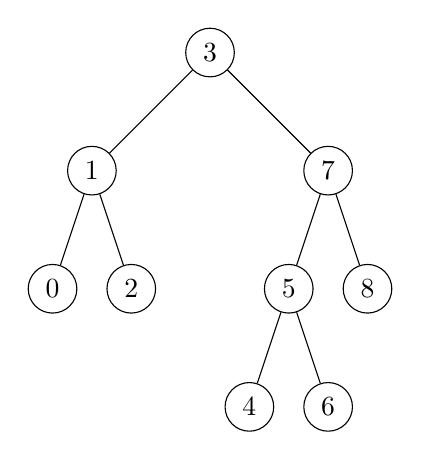
\begin{tikzpicture}
      [level 1/.style={sibling distance=30mm},
       level 2/.style={sibling distance=15mm},
       level 2/.style={sibling distance=10mm}]
      \tikzstyle{every node}=[circle,draw]
      \node{3}
      child{
        node{1}
        child{node{0}}
        child{node{2}}
      }
      child{
        node{7}
        child{
          node{5}
          child{node{4}}
          child{node{6}}
        }
        child{node{8}}
      };
    \end{tikzpicture} \hspace{4mm}
    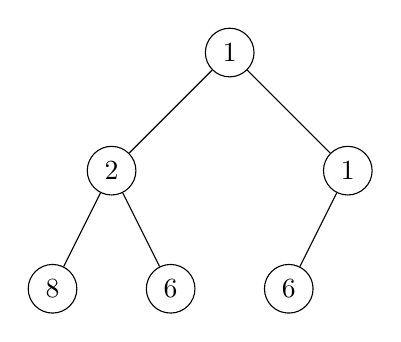
\begin{tikzpicture}
      [level 1/.style={sibling distance=30mm},
       level 2/.style={sibling distance=15mm}]
      \tikzstyle{every node}=[circle,draw]
      \node{1}
      child{
        node{2}
        child{node{8}}
        child{node{6}}
      }
      child{
        node{1}
        child{node{6}}
        child[missing]{node{k}}
      }
      ;
    \end{tikzpicture} \hspace{4mm}
    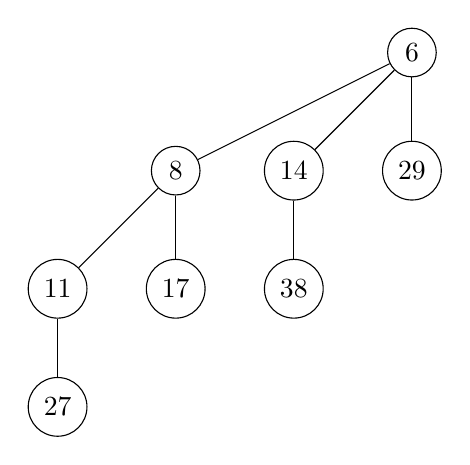
\begin{tikzpicture}[grow via three points={%
        one child at (0,-1.5) and two children at (0,-1.5) and (-1.5,-1.5)}]
      \tikzstyle{every node}=[circle,draw]
      \node at (0,0) {6}
      child{node{29}}
      child{
        node{14}
        child{
          node{38}
        }
      }
      child{
        node{8}
        child{node{17}}
        child{
          node{11}
          child{node{27}}
        }
      }
      ;
    \end{tikzpicture}
  \end{center}
  \caption{A binary search tree (on the left), a binary min-heap (in
    the middle), and a binomial tree of rank $3$ (on the right).}
  \label{fig:trees}
\end{figure}

Algorithms can be typeset as pseudo-code as exemplified in
Algorithm~\ref{algo:demo}: study its \LaTeX\ source code.

\begin{algorithm}[t]
  \begin{algorithmic}[1]  % comment [1] away to drop the line numbers
    \STATE \Function $f(n)$
    \IF[optional comment]{$n < 0$}
      \STATE $n \IsAssigned -2 \cdot n$ \COMMENT{optional comment}
    \ELSE[$n \geq 0$]
      \STATE $n \IsAssigned  3 \cdot n$
    \ENDIF
    \WHILE[optional comment]{$n > 0$}
      \STATE $n \IsAssigned n-1$
    \ENDWHILE
    \RETURN $n$
  \end{algorithmic}
  \caption{Silly algorithm}
  \label{algo:demo}
\end{algorithm}

If you are not sure whether you will stick to your current choice of
notation or terminology, then introduce a new (possibly parametric)
command.  For example, upon
\begin{center}
  \verb|\newcommand{\Cardinality}[1]{\left\lvert#1\right\rvert}|
\end{center}
the formula \verb|$\Cardinality{S}$| typesets the cardinality of set
$S$ as $\Cardinality{S}$ with autosized vertical bars and proper
spacing, but upon changing the definition of that parametric command
to
\begin{center}
  \verb|\newcommand{\Cardinality}[1]{\# #1}|
\end{center}
and recompiling, the formula \verb|$\Cardinality{S}$| typesets the
cardinality of set $S$ as $\#S$.
%
Similarly, upon
\begin{center}
  \verb|\newcommand{\MiniZinc}{\textit{Mini\-Zinc}}|
\end{center}
the text \verb|\MiniZinc\| typesets into \textit{MiniZinc},
hyphenation being only possible in the middle, but upon changing the
definition of that non-parametric command to
\begin{center}
  \verb|\newcommand{\MiniZinc}{\textsc{Mini\-Zinc}}|
\end{center}
and recompiling, the text \verb|\MiniZinc\| typesets into
\textsc{MiniZinc}.
%
You can thus obtain an arbitrary number of changes in the document
with a \emph{constant}-time change in its source code, rather than
having to perform a \emph{linear}-time find-and-replace operation
within the source code, which is painstaking and error-prone.  The
imported file \texttt{macros.tex} has a lot of useful predefined
commands about mathematics, CP, \Gecode, modelling, \MiniZinc, and
algorithms.

Use commands on positioning (such as \verb|\hspace|, \verb|\vspace|,
and \verb|\noindent|) and appearance (such as \verb|\small| for
reducing the font size, and \verb|\textit| for italics) very
sparingly, and ideally only in (parametric) commands, as the very idea
of mark-up languages such as \LaTeX\ is to let the class designer
(usually a trained professional typesetter) decide on where things
appear and how they look.  For example, \verb|\emph| (for emphasis)
compiles (outside italicised environments, such as \texttt{theorem})
into \textit{italics} under the \texttt{article} class used for this
document, but it may compile into \textbf{boldface} under some other
class.
\begin{center}
  \textbf{If you do not (need to) worry about \emph{how} things look, \\
    then you can fully focus on \emph{what} you are trying to
    express!}
\end{center}

Note that \emph{no} absolute numbers are used in the \LaTeX\ source
code for any of the references inside this document.  For ease of
maintenance, \verb|\label| is used for giving a label to something
that is automatically numbered (such as an algorithm, equation,
figure, footnote, item, line, part, section, subsection, or table),
and \verb|\ref| is used for referring to a label.  An item in the
bibliography file is referred to by \verb|\cite| instead.  Upon
changing the text, it suffices to recompile, once or twice, and
possibly to run BibTeX again, in order to update all references
consistently.

Always write
%
\verb| Table|$\sim$\verb|\ref{tab:maths} |
%
instead of
%
\verb| Table \ref{tab:maths}|,
%
by using the non-breaking space (which is typeset as the tilde $\sim$)
instead of the normal space, because this avoids that a
cross-reference is spread across a line break, as for example in
``Table \ref{tab:maths}'', which is considered poor typesetting.

The rules of English for how many spaces to use before and after
various symbols are given in Table~\ref{tab:spacing}.  Beware that
they may be very different from the rules in your native language.

\begin{table}[t]
  \centering
  \begin{tabular}{cc|c|c}
    \toprule
    \multicolumn{2}{c}{} & \multicolumn{2}{l}{number of spaces after} \\
    \cmidrule{3-4}
    \multicolumn{2}{c}{} & 0 & 1 \\
    \midrule
    \multirow{2}{*}{number of spaces before} & 0 & / - & , : ; . ! ?
    ) ] \} ' '' \% \\
    \cmidrule{2-4}
    & 1 & ( [ \{ ` `` & -- (\emph{n}-dash) --- (\emph{m}-dash) \\
    \bottomrule
  \end{tabular}
  \caption{Spacing rules of English}
  \label{tab:spacing}
\end{table}

\vfill

\noindent
\handpoint\ Feel free to report to the head teacher any other features
that you would have liked to see discussed and exemplified in this
template document.
}

\end{document}

%%% Local Variables:
%%% mode: latex
%%% TeX-master: t
%%% End:
